%!TEX program = xelatex
\documentclass[8pt, landscape, a4paper]{extarticle}

% --- 核心宏包 ---
\usepackage[UTF8, fontset=fandol]{ctex}
\usepackage[margin=0.8cm, top=1cm, bottom=1.3cm]{geometry}
\usepackage{multicol}
\usepackage{xcolor}
\usepackage{tcolorbox}
\usepackage{enumitem}
\usepackage{amsmath}
\usepackage{amssymb}
\usepackage{fontspec}
\usepackage{tikz}
\usetikzlibrary{arrows.meta, shapes}

% --- 去掉页码 ---
\pagestyle{empty}

% --- 颜色定义 (Orange 主题) ---
\definecolor{headerblue}{RGB}{230, 126, 34}    % Carrot
\definecolor{navcolor}{RGB}{211, 84, 0}        % 导航橙
\definecolor{intuitioncolor}{RGB}{41, 128, 185}% 直觉蓝
\definecolor{accentcolor}{RGB}{192, 57, 43}    % 强调红
\definecolor{section2}{RGB}{22, 160, 133}      % 绿色
\definecolor{dividergray}{RGB}{220, 220, 220}

% --- 全局设置 ---
\setlength{\parindent}{0pt}
\setlength{\columnsep}{0.4cm} 
\linespread{1.1} 

% --- 列表样式 ---
\setlist[itemize]{leftmargin=1.2em, nosep, itemsep=2pt, topsep=2pt, label=$\textcolor{headerblue}{\vcenter{\hbox{\tiny$\bullet$}}}$ }
\setlist[description]{leftmargin=0.2em, style=sameline, nosep, itemsep=2pt, font=\bfseries}

% --- Box 样式 ---
\newtcolorbox{mybox}[2][]{%
  colback=white,
  colframe=#2,
  coltitle=white,
  boxrule=1pt,   
  arc=2mm,                 
  left=4pt, right=4pt, top=3pt, bottom=3pt, 
  toptitle=3pt, bottomtitle=3pt, 
  fonttitle=\bfseries\sffamily\large,
  title={#1},
  after skip=5pt          
}

% --- 自定义命令 ---
\newcommand{\subt}[1]{{\vspace{2pt}\textbf{\large \textcolor{black}{#1}}}}

\newcommand{\boxdesc}[1]{%
    \textit{\small \textcolor{gray}{#1}}%
    \par\vspace{2pt}%
    {\color{dividergray}\hrule height 0.5pt}%
    \vspace{2pt}%
}

\newcommand{\sepline}{%
    \par \vspace{3pt}%
    {\color{dividergray}\hrule height 0.5pt}%
    \par \vspace{3pt}%
}

% 公式间距
\setlength{\abovedisplayskip}{3pt}
\setlength{\belowdisplayskip}{3pt}

\begin{document}

% --- 页眉 ---
\begin{center}
    {\Huge \textbf{\sffamily \textcolor{headerblue}{随机微积分 Stochastic Calculus Cheat Sheet}}} \\
    \vspace{0.2cm}
    {\large \texttt{Calculus for the Unpredictable: Ito's Lemma and Beyond}}
\end{center}

% --- 开始四栏布局 ---
\begin{multicols*}{4}

% === 第一栏 ===

\begin{mybox}[️ 场景导航 (Use Cases)]{navcolor}
    \boxdesc{遇到什么问题 $\to$ 用什么工具}
    \begin{itemize}[itemsep=2pt]
        \item \textbf{股票期权定价} $\to$ Black-Scholes 方程
        \item \textbf{噪声系统建模} $\to$ 随机微分方程 (SDE)
        \item \textbf{强化学习 (RL)} $\to$ 策略梯度 / 随机探索
        \item \textbf{扩散模型 (AI)} $\to$ Langevin 动力学
        \item \textbf{风险管理} $\to$ Value at Risk (VaR)
        \item \textbf{信号处理} $\to$ 卡尔曼滤波
    \end{itemize}
\end{mybox}

\begin{mybox}[1. 布朗运动 (Brownian Motion)]{headerblue}
    \boxdesc{随机游走 $W_t$}
    
    \subt{定义 (维纳过程)}
    \begin{itemize}
        \item $W_0 = 0$。
        \item \textbf{独立增量}: $W_{t+s} - W_t$ 独立于过往。
        \item \textbf{正态增量}: $W_{t+s} - W_t \sim N(0, s)$。
        \item \textbf{路径性质}: 处处连续,但\textbf{处处不可导}。
    \end{itemize}
    \sepline
    
    \subt{二次变差 (Quadratic Variation)}
    $$ [W, W]_t = t $$
    \textit{直觉: $(dW_t)^2 = dt$。这是随机微积分与普通微积分的核心区别。}
    \textbf{协变差}: $[W^i, W^j]_t = \delta_{ij} t$ (独立时为0)。
\end{mybox}

\begin{mybox}[2. 伊藤积分 (Ito Integral)]{headerblue}
    \boxdesc{对随机过程积分}
    
    \subt{定义}
    $$ I(t) = \int_0^t \Delta_s dW_s $$
    取区间\textbf{左端点}进行黎曼和逼近。
    \begin{itemize}
        \item \textbf{鞅性质 (Martingale)}: 期望不变 $E[I(t)] = 0$。
        \item \textbf{伊藤等距}: $E[(\int \Delta dW)^2] = E[\int \Delta^2 dt]$。
    \end{itemize}
    \sepline
    
    \subt{Stratonovich 积分}
    取区间\textbf{中点}。符合普通微积分链式法则,但不是鞅。
    \textit{物理中常用 Stratonovich,金融中常用 Ito。}
\end{mybox}

\columnbreak

% === 第二栏 ===

\begin{mybox}[3. 伊藤引理 (Ito's Lemma)]{headerblue}
    \boxdesc{随机微积分的链式法则}
    
    \subt{公式}
    如果 $X_t$ 服从 $dX_t = \mu dt + \sigma dW_t$,且 $f(t, x)$ 是光滑函数,则 $Y_t = f(t, X_t)$ 服从:
    $$ df = (\frac{\partial f}{\partial t} + \mu \frac{\partial f}{\partial x} + \frac{1}{2} \sigma^2 \frac{\partial^2 f}{\partial x^2}) dt + \sigma \frac{\partial f}{\partial x} dW_t $$
    \sepline
    
    \subt{直觉推导 (泰勒展开)}
    $$ df \approx f_t dt + f_x dX + \frac{1}{2} f_{xx} (dX)^2 $$
    代入 $(dX)^2 = \sigma^2 dt$ (忽略 $dt^2$ 和 $dt dW$)。
    \textit{关键项: $\frac{1}{2} \sigma^2 f_{xx} dt$ 是普通微积分没有的“凸性修正”。}
    \textbf{乘积法则}:
    $$ d(X_t Y_t) = X_t dY_t + Y_t dX_t + dX_t dY_t $$
\end{mybox}

\begin{mybox}[4. 随机微分方程 (SDE)]{headerblue}
    \boxdesc{带噪声的 ODE}
    
    \subt{一般形式}
    $$ dX_t = \mu(t, X_t) dt + \sigma(t, X_t) dW_t $$
    \begin{itemize}
        \item $\mu$: 漂移项 (Drift, 确定性趋势)。
        \item $\sigma$: 扩散项 (Diffusion, 随机波动)。
    \end{itemize}
    \sepline
    
    \subt{几何布朗运动 (GBM)}
    股票价格模型:
    $$ dS_t = \mu S_t dt + \sigma S_t dW_t $$
    解: $S_t = S_0 \exp((\mu - \frac{1}{2}\sigma^2)t + \sigma W_t)$。
    \textit{注意: $\frac{1}{2}\sigma^2$ 的修正项。}
    \sepline
    
    \subt{Ornstein-Uhlenbeck 过程 (OU)}
    均值回归过程 (Mean-Reverting)。
    $$ dX_t = \theta (\mu - X_t) dt + \sigma dW_t $$
    \begin{itemize}
        \item $\theta$: 回归速度。$\mu$: 长期均值。
        \item \textbf{应用}: 利率模型 (Vasicek), 配对交易。
        \item 解是高斯过程,方差有界。
    \end{itemize}
\end{mybox}

\columnbreak

% === 第三栏 ===

\begin{mybox}[5. Black-Scholes 方程]{headerblue}
    \boxdesc{金融界的 $E=mc^2$}
    
    \subt{偏微分方程 (PDE)}
    期权价格 $V(S, t)$ 满足:
    $$ \frac{\partial V}{\partial t} + \frac{1}{2}\sigma^2 S^2 \frac{\partial^2 V}{\partial S^2} + rS \frac{\partial V}{\partial S} - rV = 0 $$
    \sepline
    
    \subt{费曼-卡茨公式 (Feynman-Kac)}
    建立了 PDE 和 SDE 的桥梁。
    PDE 的解等于 SDE 路径的期望。
    $$ V(S, t) = E[e^{-r(T-t)} \text{Payoff}(S_T)] $$
    \textit{启示: 求解 PDE 可以通过蒙特卡洛模拟 SDE 来实现。}
    \textbf{希腊字母}: $\Delta = \partial V / \partial S$ (对冲比率), $\Gamma = \partial^2 V / \partial S^2$ (凸性)。
\end{mybox}

\begin{mybox}[6. 测度变换 (Girsanov)]{headerblue}
    \boxdesc{改变概率的世界}
    
    \subt{风险中性测度 (Risk-Neutral)}
    在真实世界 $P$ 下,股票有漂移 $\mu$。
    通过 Girsanov 定理换到测度 $Q$,使得股票漂移变为无风险利率 $r$。
    \textit{在 $Q$ 测度下,所有资产的贴现价格都是鞅。}
    \sepline
    
    \subt{鞅表示定理}
    任何 $Q$-鞅都可以表示为布朗运动的积分。
    \textit{意义: 完备市场中,任何衍生品都可以被复制 (Hedging)。}
    \textbf{Novikov 条件}: 保证 $Z_t$ 是真正的鞅。
    $$ E[\exp(\frac{1}{2} \int_0^T \theta_s^2 ds)] < \infty $$
\end{mybox}

\begin{mybox}[7. Python / QuantLib 实战]{headerblue}
    \boxdesc{代码工具箱}
    \begin{itemize}
        \item \textbf{模拟 GBM}:
        \texttt{dt = T/N; dW = np.random.normal(0, sqrt(dt), N)}
        \texttt{S = S0 * exp(cumsum(...))}
        \item \textbf{解 SDE}: \texttt{sdeint} 库。
        \item \textbf{期权定价}: \texttt{QuantLib}。
    \end{itemize}
\end{mybox}

\columnbreak

% === 第四栏 ===

\begin{mybox}[8. 高阶应用 (Advanced)]{headerblue}
    \boxdesc{AI 与 物理}
    
    \subt{朗之万动力学 (Langevin)}
    $$ dX_t = -\nabla U(X_t) dt + \sqrt{2} dW_t $$
    平稳分布是玻尔兹曼分布 $p(x) \propto e^{-U(x)}$。
    \textit{应用: 贝叶斯采样 (MCMC),扩散模型 (Stable Diffusion)。}
    \sepline
    
    \subt{随机控制 (Stochastic Control)}
    HJB 方程 (Hamilton-Jacobi-Bellman)。
    在随机环境下寻找最优策略。
\end{mybox}

\vspace*{\fill}

\begin{mybox}[ 核心直觉 (Intuition)]{intuitioncolor}
    \boxdesc{“噪音也是信号。”}
    
    % TikZ 矢量图: 布朗运动路径 vs 光滑路径
    \begin{center}
    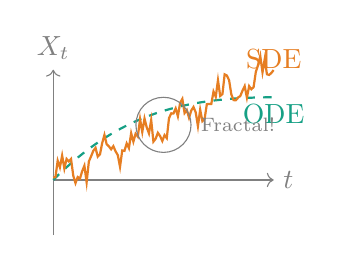
\begin{tikzpicture}[scale=0.7]
        \draw[->, gray] (0,0) -- (4,0) node[right] {$t$};
        \draw[->, gray] (0,-1) -- (0,2) node[above] {$X_t$};
        
        % 光滑路径 (ODE)
        \draw[thick, section2, dashed] (0,0) to[out=45, in=180] (4, 1.5);
        \node[section2] at (4, 1.2) {ODE};
        
        % 随机路径 (SDE)
        \draw[thick, headerblue] plot[domain=0:4, samples=100] (\x, {0.5*\x + 0.2*rand + 0.2*sin(500*\x)}); 
        % 注意: TikZ 的 rand 是伪随机,这里只是示意 jaggedness
        \node[headerblue] at (4, 2.2) {SDE};
        
        % 放大镜效果
        \draw[gray] (2, 1) circle (0.5cm);
        \node[right, gray, font=\scriptsize] at (2.5, 1) {Fractal!};
    \end{tikzpicture}
    \end{center}

    \hspace{1em}随机微积分处理的是\textbf{不可微}的函数。普通微积分假设曲线无限放大后是直线,而布朗运动无限放大后依然是锯齿。
    \vspace{4pt}
    
    \subt{三大核心视角}
    \begin{itemize}[itemsep=4pt]
        \item \textbf{二阶效应不可忽略}: 
        在普通微积分中,$(dx)^2$ 是高阶无穷小,可以扔掉。但在随机微积分中,$(dW)^2 = dt$,是一阶无穷小,必须保留。这就是伊藤项的来源。
        
        \item \textbf{鞅 (Martingale)}: 
        公平的赌局。如果你无法预测未来的增量 (期望为0),那么这个过程就是鞅。有效市场假说认为股价本质上是鞅。
        
        \item \textbf{噪声驱动}: 
        SDE 告诉我们,系统的演化 = 确定性的物理定律 (Drift) + 随机的热涨落 (Diffusion)。
    \end{itemize}
    
    \vspace{6pt}
    \centering\textit{\footnotesize 上帝掷骰子,伊藤算出了骰子的轨迹。}
\end{mybox}

\end{multicols*}

\end{document}
